% $Header$
% $Author: fager $
% $Date: 2004-10-21 20:59:19 +0200 (Thu, 21 Oct 2004) $
% $Revision: 223 $
% $Log$
% Revision 1.2  2004/10/21 18:59:06  fager
% Version logging added. Comments from KA implemented.
%
\section{Model representation using netlists}\label{sec:mna}
So far, the description has been focused on handling measured
S-parameter data originating from TouchStone files etc. However,
in many applications it is also desired to handle the S-parameters
of an ideal electrical circuit diagram. This is typically the case
in modelling applications, where the parameters of a model is
determined by minimizing the difference between the S-parameters
generated by the model and the measured ones.

\subsection{Netlist format and importing}
The circuit shown in \figref{Circuit} will hereafter serve as an
example.

\begin{figure}[htbf]
    \centering
  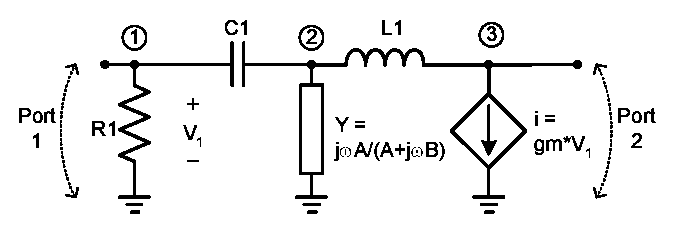
\includegraphics[scale=0.85]{Figures/Circuit.eps}
  \caption{Example circuit.}\label{fig:Circuit}
\end{figure}

Electrical circuits are entered into Milou by means of a
\emph{netlist} file, similar to the ones used in Spice. The
expressions shown in \tabref{Netlist} are recognized by the Milou
netlist parser:

\begin{table}[htbf]
    \centering
  \caption{Valid netlist expressions.}\label{tab:Netlist}
    \begin{minipage}{\textwidth}
    \centering
    \begin{small}
    \begin{tabular}{l|l}
    % after \\: \hline or \cline{col1-col2} \cline{col3-col4} ...
    Component & Netlist expression\\
    \hline
    Resistance & \verb"R value"\footnote{A \emph{value} can be either a numeric value or a parameter name.}\verb" node1 node2"\\
    Conductance & \verb"G value node1 node2"\\
    Capacitance & \verb"C value node1 node2"\\
    Inductance & \verb"L value node1 node2"\\
    General admittance & \verb"X expression"\footnote{An \emph{expression} can include an arbitrary algebraic expression. $s$ should be used instead of $j\omega$. Other names that are not recognized functions will be considered user parameters.} \verb" node1 node2"\\
    Transconductance& \verb"VCCS value node1+ node2+ node1- node2-"\\
    Transcond. with $\tau$& \verb"VCCSD value node1+ node2+ node1- node2-"\\
    Gyrator & \verb"GY value node1+ node2+ node1- node2-"\\
    General transcond. & \verb"X2 expression node1+ node2+ node1- node2-"\\
    Port & \verb"P portname node1 node 2"\\
    Comment & \verb"% Comment text" \\
    \hline
    \end{tabular}
    \end{small}
    \end{minipage}
\end{table}

The netlist corresponding to the circuit in \figref{Circuit}
becomes (\verb"circuit.net"):
\begin{small}
\begin{verbatim}
    % Example circuit
    R R1 1 0
    C C1 1 2
    X s*A/(A+s*B) 2 0
    L L1 2 3
    VCCS gm 1 3 0 0
    P P1 1 0
    P P2 3 0
\end{verbatim}
\end{small}

The netlist can now be imported into Milou by using the
\verb"read_netlist" function,
\begin{small}
\begin{verbatim}
    >> model = read_netlist(mna,'doc/Usersmanual/circuit.net')
    Admittance matrix:
        '+1/(R1)+s*C1'    '-s*C1'                 []
        '-s*C1'           [1x26 char]    '-1/(s*L1)'
        '+gm'             '-1/(s*L1)'    '+1/(s*L1)'
    Parameters:
        'R1'
        'C1'
        'A'
        'B'
        'L1'
        'gm'
    Parameter types:
        'R'
        'C'
        'X'
        'X'
        'L'
        'VCCS'
    Frequencies
    Partials
        1
        1
        1
        1
        1
        1
\end{verbatim}
\end{small}

The output variable \verb"model" is now an \verb"mna" object. mna
stands for \emph{modified nodal admittance}, which is the type of
matrix normally used to represent circuits in simulators. Milou
currently uses the ordinary nodal admittance matrix for
representing circuits\footnote{The modified nodal admittance
matrix uses a different representation of components that may
present infinite conductance, e.g. inductances at low frequency,
and thus provides better numerical stability.}. It is, by the way,
shown in the first part of the displayed \verb"mna" object
information displayed above.

The next thing displayed is the list of parameters. These are the
unique parameter names found in the netlist. The order in which
the parameters appear is important when, at a later stage, their
values should be assigned. The parameter names can also be
accessed by the \verb"params" command,
\begin{small}
\begin{verbatim}
    >> params(model)
    ans =
        'R1'    'C1'    'A'    'B'    'L1'    'gm'
\end{verbatim}
\end{small}

Next in the results displayed is the types associated with the parameters.
This is not applicable for parameters defined in \verb"X" or
\verb"X2" elements.

Finally is a list of partial derivatives that are used for
calculating sensitivities. This feature is, however, not treated
in this manual text.

\subsection{Evaluation of the model X-parameters}
Before it is possible to assign numbers to the model parameter and
evaluate its X-parameters, one needs to specify the frequencies
used for consequent calculations. The reason that the frequencies
are entered separately is to speed up the X-parameter evaluations
later. The frequencies are assigned to the \verb"mna"-object using
the \verb"freq" command,
\begin{small}
\begin{verbatim}
    >> model = freq(model,msp.freq);
\end{verbatim}
\end{small}
where the same frequencies as in the previous measurement examples
have been used.

It is now possible to evaluate the model for any set of parameters
using a call to either the \verb"calc" or the \verb"reduce"
functions. The model parameter values should be arranged in a
vector with the order being the same as described above.
\begin{small}
\begin{verbatim}
    >> R1 = 100;C1 = 1e-12;A = 0.7e-12;B = 2e-12;
    >> L1 = 1e-9; gm = 1e-3;
    >> model_params = [R1,C1,A,B,L1,gm];
\end{verbatim}
\end{small}

Once the parameters have been defined it is possible to calculate
either the full $N$-by-$N$ matrix, where $N$ is the number of
nodes, or a reduced matrix describing the circuit as observed at
the ports that were defined in the netlist.

The first case is evaluated by using the \verb"calc" function,
\begin{small}
\begin{verbatim}
    >> calc(model,model_params)
    xparam-object
        type:  Y
        reference: 50
        ports: 3
        elements:  101
\end{verbatim}
\end{small}
The resulting object is, for our three-node example an 3-by-3
Y-type \verb"xparam" object.

The function \verb"reduce" is used in a similar fashion to
calculate the port-reduced Z-parameters,
\begin{small}
\begin{verbatim}
    >> xp_model = reduce(model,model_params)
    xparam-object
        type:  Z
        reference: 50
        ports: 2
        elements:  101
\end{verbatim}
\end{small}
Note that the resulting object is a 2-by-2 Z-type \verb"xparam"
object, which can be handled in exactly the same manner as the
measurements were used before.
